%%%%%%%%%%%%%%%%%%%%%%%%%%%%%%%%%%%%%%%%%%%%%%%%%%%%%%%%%%%%%%%%%%%%%%%%%%%%%%%
%% Resource-Normalized Scaling Laws for Byzantine Consensus
%% Peniak B.O., Liubinskyj B.B.
%%
%% COMPILE WITH pdflatex (T2A fontenc + babel). NOT xelatex / lualatex.
%%   pdflatex paper3 && pdflatex paper3
%% Bibliography is a manual `thebibliography' environment: NO bibtex / biblatex.
%%%%%%%%%%%%%%%%%%%%%%%%%%%%%%%%%%%%%%%%%%%%%%%%%%%%%%%%%%%%%%%%%%%%%%%%%%%%%%%

\documentclass[12pt]{article}
\usepackage{MMC}

%%%%%%%%%%%%%%%%%%%%%%%%%%%%%%%%%%%%%%%%%%%%%%%%%%%%%%%%%%%%%%%%%%%%%%%%%%%%%%%
%% macros.tex -- symbols of the model.
%% Rule: this file defines NOTATION only. Numeric results live in numbers.tex
%% and are generated by experiments/analysis/emit_numbers_tex.py.
%% Never hard-code a measured number in a section file.
%%%%%%%%%%%%%%%%%%%%%%%%%%%%%%%%%%%%%%%%%%%%%%%%%%%%%%%%%%%%%%%%%%%%%%%%%%%%%%%

%--------------------------------------------------------------- primary symbols
\newcommand{\n}{n}                  % validator count
\newcommand{\cc}{c}                 % client concurrency (number of senders)
\newcommand{\q}{q}                  % per-validator CPU quota (cores)
\newcommand{\w}{w}                  % detection window length (epochs)
\newcommand{\kf}{k}                 % number of faulty validators

%------------------------------------------------------------------ throughput
\newcommand{\TPS}{\mathrm{TPS}}
\newcommand{\TPSn}{\widetilde{\mathrm{TPS}}}   % resource-normalized throughput
\newcommand{\Tzero}{T_{0}}
\newcommand{\gfun}{g}                          % client-concurrency factor
\newcommand{\csat}{c^{\ast}}                   % saturation concurrency
\newcommand{\ahat}{\hat{\alpha}}               % single-factor (confounded) exponent
\newcommand{\bhat}{\hat{\beta}}
\newcommand{\ghat}{\hat{\gamma}}

%-------------------------------------------------------------------- detection
\newcommand{\Bhat}{\hat{B}}
\newcommand{\pd}{p_{d}}
\newcommand{\pf}{p_{f}}
\newcommand{\pmiss}{p_{\mathrm{miss}}}
\newcommand{\neff}{n_{\mathrm{eff}}}
\newcommand{\thr}{\tau}                        % override threshold

%----------------------------------------------------------------------- sizing
\newcommand{\Dpk}{D_{\mathrm{peak}}}
\newcommand{\epsp}{\varepsilon_{p}}
\newcommand{\epss}{\varepsilon_{s}}
\newcommand{\nmin}{n_{\min}}
\newcommand{\nmax}{n_{\max}}
\newcommand{\nopt}{n^{\ast}}
\newcommand{\Cost}{\mathrm{Cost}}
\newcommand{\Feas}{\mathcal{F}}

%------------------------------------------------------------------- statistics
\newcommand{\E}{\mathbb{E}}
\newcommand{\Prob}{\mathbb{P}}
\newcommand{\Var}{\mathrm{Var}}
\newcommand{\Cov}{\mathrm{Cov}}
\newcommand{\zq}[1]{z_{#1}}
\newcommand{\PI}{\mathrm{PI}}

%------------------------------------------------------------------- shorthands
\newcommand{\eqdef}{\mathrel{\mathop:}=}
\newcommand{\RNM}{RNM}
\newcommand{\ie}{i.\,e.}
\newcommand{\eg}{e.\,g.}

%%%%%%%%%%%%%%%%%%%%%%%%%%%%%%%%%%%%%%%%%%%%%%%%%%%%%%%%%%%%%%%%%%%%%%%%%%%%%%%
%% numbers.tex -- AUTO-GENERATED. DO NOT EDIT BY HAND.
%%
%% Regenerate with:
%%     python experiments/analysis/emit_numbers_tex.py \
%%            --in data/processed --out numbers.tex
%%
%% Until the experimental campaign has been run, every macro below expands to a
%% visible \TODO marker, so that an unfilled number cannot silently reach the
%% submitted PDF.
%%%%%%%%%%%%%%%%%%%%%%%%%%%%%%%%%%%%%%%%%%%%%%%%%%%%%%%%%%%%%%%%%%%%%%%%%%%%%%%

%--- bi-factor calibration (X1, X3) -------------------------------------------
\newcommand{\resBeta}{\TODO{beta}}
\newcommand{\resBetaSE}{\TODO{se(beta)}}
\newcommand{\resGamma}{\TODO{gamma}}
\newcommand{\resGammaSE}{\TODO{se(gamma)}}
\newcommand{\resCsat}{\TODO{c*}}
\newcommand{\resTheta}{\TODO{theta}}
\newcommand{\resTzero}{\TODO{T0}}
\newcommand{\resRsq}{\TODO{R2}}
\newcommand{\resSigmaRes}{\TODO{sigma}}

%--- confounding check (Theorem 1) --------------------------------------------
\newcommand{\resLambda}{\TODO{lambda}}
\newcommand{\resAlphaHat}{\TODO{alpha-hat}}
\newcommand{\resAlphaPred}{\TODO{gamma*lambda-beta}}

%--- q-invariance (X2) ---------------------------------------------------------
\newcommand{\resBetaQlow}{\TODO{beta(q=0.20)}}
\newcommand{\resBetaQmid}{\TODO{beta(q=0.25)}}
\newcommand{\resBetaQhigh}{\TODO{beta(q=0.33)}}
\newcommand{\resQinvP}{\TODO{p-value}}

%--- WAN degradation (X4) ------------------------------------------------------
\newcommand{\resBetaRttZero}{\TODO{beta(0ms)}}
\newcommand{\resBetaRttHigh}{\TODO{beta(200ms)}}

%--- detector characterisation (X5) --------------------------------------------
\newcommand{\resPd}{\TODO{p_d}}
\newcommand{\resPf}{\TODO{p_f}}
\newcommand{\resRho}{\TODO{rho}}
\newcommand{\resAuc}{\TODO{AUC}}

%--- prediction-interval coverage (X7) -----------------------------------------
\newcommand{\resCovNinety}{\TODO{cov90}}
\newcommand{\resCovNinetyFive}{\TODO{cov95}}
\newcommand{\resHoldoutN}{\TODO{n_holdout}}

%--- sizing ablation (X8) ------------------------------------------------------
\newcommand{\resNminCase}{\TODO{n_min}}
\newcommand{\resNmaxCase}{\TODO{n_max}}
\newcommand{\resNoptCase}{\TODO{n*}}
\newcommand{\resCostLinear}{\TODO{cost-linear}}
\newcommand{\resCostSingle}{\TODO{cost-single-factor}}
\newcommand{\resCostUsl}{\TODO{cost-usl}}
\newcommand{\resCostOurs}{\TODO{cost-ours}}

%--- campaign metadata ---------------------------------------------------------
\newcommand{\resNmaxMeasured}{\TODO{n_max measured}}
\newcommand{\resTotalRuns}{\TODO{runs}}
\newcommand{\resCoreHours}{\TODO{core-hours}}


%%%%%%%%%%%%%%%%%%%%%%%%%%%%%%%%%% METADATA (EN) %%%%%%%%%%%%%%%%%%%%%%%%%%%%%%%

\title[Resource-Normalized Scaling Laws for BFT Consensus]{Resource-Normalized
Scaling Laws for Byzantine Consensus: Chance-Constrained Validator-Set Sizing
from Commodity-CI Measurements}

\author[Peniak B.\,O.]{Peniak B.\,O., Liubinskyj B.\,B.}

\organization{%
\address{1}Lviv Polytechnic National University\\
12 S.~Bandera str., 79013, Lviv, Ukraine\\
\address{2}Institute of Applied Mathematics and Fundamental Sciences}

\email{bohdan.o.peniak@lpnu.ua}

\received{xx xxxxx 20xx}

\abstract{%
\textbf{Problem.} Sizing the validator set of a permissioned Byzantine Fault
Tolerant (BFT) network for a national-scale e-governance workload requires
reconciling two opposing forces: consensus throughput degrades as the validator
count~$\n$ grows, whereas the statistical power of fault detection improves
with~$\n$. Published single-factor scaling coefficients are moreover not
reproducible across testbeds.
%
\textbf{Contributions.} (1)~An \emph{identifiability theorem} showing that the
single-factor exponent converges to $\ahat=\gamma\lambda-\beta$, where
$\lambda$ describes how client concurrency was scaled with the network, so that
$\ahat$ is a confounded projection rather than an intrinsic protocol property;
(2)~a \emph{resource-normalized measurement} protocol fixing the per-validator
CPU quota~$\q$ independently of~$\n$, which is what makes the required
factorial design feasible on a single commodity host; (3)~calibrated lognormal
\emph{prediction intervals} validated by empirical coverage; (4)~a
\emph{chance-constrained sizing problem} and a \emph{feasibility-window
theorem} proving that the admissible validator counts form a closed interval
$[\nmin,\nmax]$ computable in $O(\log \n)$, an empty interval certifying that
no validator count meets the requirement.
%
\textbf{Validation.} The full campaign executes inside a public
continuous-integration workflow on a single four-core runner, covering
$\n\in\{4,\dots,16\}$, client concurrency $\cc\in[1,64]$, emulated wide-area
latency, and omission/duplication fault injection with an empirically
characterized detector.
%
\keywords{Byzantine fault tolerance, consensus, scaling law, capacity planning,
chance-constrained optimization, e-governance}
\MSC{68M14, 68W20, 90C15, 62J02}
\udk{004.75:519.2}
}

%%%%%%%%%%%%%%%%%%%%%%%%%%%%%%%%% METADATA (UKR) %%%%%%%%%%%%%%%%%%%%%%%%%%%%%%%

\titleUkr[Ресурсно-нормовані закони масштабування BFT-консенсусу]{РЕСУРСНО-НОРМОВАНІ
ЗАКОНИ МАСШТАБУВАННЯ BFT-КОНСЕНСУСУ: ІМОВІРНІСНО-ОБМЕЖЕНЕ ВИЗНАЧЕННЯ РОЗМІРУ
МНОЖИНИ ВАЛІДАТОРІВ ЗА ВИМІРЮВАННЯМИ НА ТИПОВІЙ CI-ІНФРАСТРУКТУРІ}

\authorUkr[Пеняк Б.\,О.]{Пеняк Б.\,О., Любінський Б.\,Б.}

\organizationUkr{%
Національний університет <<Львівська політехніка>>\\
вул.~С.~Бандери, 12, 79013, Львів, Україна}

\abstractUkr{%
Запропоновано метод визначення розміру множини валідаторів BFT-мережі для
навантажень електронного урядування, який поєднує дві протилежні залежності:
пропускна здатність консенсусу спадає зі зростанням кількості валідаторів~$\n$,
тоді як статистична потужність виявлення візантійської поведінки зростає з~$\n$.
%
Основні результати: 1)~протокол ресурсно-нормованих вимірювань, що фіксує
CPU-квоту~$\q$ на валідатор незалежно від~$\n$ і робить показник масштабування
ідентифіковним за вимірюваннями на одному хості; 2)~двофакторний закон
$\TPS(\n,\cc)=\Tzero\,\gfun(\cc)\,\n^{-\beta}$ і теорема ідентифікованості, яка
показує, що однофакторний показник $\ahat=\gamma\lambda-\beta$ є зміщеною
проєкцією і не є внутрішньою характеристикою протоколу; 3)~лог-нормальні
прогнозні інтервали замість евристичних оцінок точності; 4)~задача визначення
розміру множини валідаторів з імовірнісними обмеженнями та теорема про вікно
допустимості, яка доводить, що множина допустимих значень~$\n$ є замкненим
інтервалом $[\nmin,\nmax]$, обчислюваним за $O(\log \n)$.
%
Увесь експериментальний цикл виконується у публічному
CI-середовищі на одному чотириядерному вузлі.
%
\keywordsUkr{візантійська відмовостійкість, консенсус, закон масштабування,
планування потужності, оптимізація з імовірнісними обмеженнями, електронне
урядування}
\udkUkr{004.75:519.2}
}

%%%%%%%%%%%%%%%%%%%%%%%%%%%%%%%%%%%% BODY %%%%%%%%%%%%%%%%%%%%%%%%%%%%%%%%%%%%%%

\begin{document}

\maketitle

\section{Introduction}
\label{sec:intro}

Permissioned Byzantine Fault Tolerant (BFT) consensus underpins a growing class
of e-governance systems: electronic voting, land and business registries,
digital identity. Deploying one at national scale requires answering a concrete
question before any node is procured: \emph{how many validators should the
network have?}

The validator count~$\n$ acts in two opposite directions. Throughput argues for
small~$\n$: every validator executes every transaction and PBFT-family
protocols exchange $O(\n^{2})$ messages per block. Safety argues for
large~$\n$: detecting a coordinated faulty minority is a statistical estimation
problem whose concentration bounds tighten exponentially in~$\n$. The two
regimes have so far been studied separately; their joint treatment is the
subject of this paper.

Two obstacles stand in the way. First, \emph{scaling exponents are not
reproducible}: published power-law fits $\TPS(\n)\propto\n^{\alpha}$ disagree in
magnitude and sometimes in sign, and our own two earlier studies are an
instance --- extrapolated to sixty validators they differ by roughly an order of
magnitude. One cause is mundane. Client-side offered concurrency is rarely held
fixed while~$\n$ is varied, since a larger network is usually driven by a larger
load generator, so the fitted exponent mixes a client-parallelism effect with
the consensus-overhead effect. Second, \emph{large testbeds are unavailable}:
calibrating a scaling law is assumed to require a testbed of the target size,
and running many validators on one host confounds consensus overhead with
contention for the host CPU --- precisely the quantity one is trying to isolate.

\paragraph{Contributions.}
The first result is central; the other three exist because it is not useful on
its own.

\begin{enumerate*}
\item \textbf{An identifiability theorem} (Section~\ref{sec:model}). If
throughput obeys $\TPS(\n,\cc)=\Tzero\,\gfun(\cc)\,\n^{-\beta}$ with $\beta>0$
and the campaign varies concurrency together with the network along a path
$\log\cc=\lambda\log\n+\mathrm{const}$, then the single-factor least-squares fit
converges in probability to $\ahat=\gamma\lambda-\beta$
(Theorem~\ref{thm:identifiability}). A positive single-factor exponent is thus
evidence about~$\lambda$, not about the protocol, and exponents from different
testbeds are incomparable unless their concurrency paths are --- which is rarely
reported.

\item \textbf{A measurement protocol that makes it usable}
(Section~\ref{sec:model}). Setting $\lambda=0$ requires a factorial design, and
on one host $\n$ validators sharing $Q$ cores receive a per-validator budget
that itself depends on~$\n$. We fix a CPU quota~$\q$ per validator irrespective
of~$\n$ and report $\TPSn=\TPS/\q$; the resulting invariance
(Statement~\ref{st:qinvariance}) is tested, not assumed.

\item \textbf{Prediction intervals validated by coverage}
(Section~\ref{sec:sizing}), replacing the average percentage error that this
literature usually reports and that cannot be checked.

\item \textbf{Sizing as a chance-constrained program}
(Section~\ref{sec:sizing}). The throughput and detection constraints move in
opposite directions, so the feasible set is a closed interval $[\nmin,\nmax]$
(Theorem~\ref{thm:window}) located in $O(\log\n)$ evaluations; an empty interval
certifies that no validator-set size satisfies the requirement.
\end{enumerate*}

We claim nothing new for the detection bound itself: it is Hoeffding's
inequality with a design-effect correction, and its role is to supply the second
constraint with parameters we measure rather than postulate.

\paragraph{Scope.}
We model throughput and detection reliability only; cryptographic design,
endpoint security and coercion resistance are outside the scope. Absolute
throughput values are specific to the constrained environment, and every claim
concerns exponents and the sizing decisions derived from them. All measurements
come from one implementation on one host, which is a real limitation;
Section~\ref{sec:case} states the cross-platform prediction that
Theorem~\ref{thm:identifiability} makes and that a second implementation can
falsify.

\section{Related work}
\label{sec:related}

\subsection{BFT consensus protocols}

Classical Practical Byzantine Fault Tolerance~\cite{castro1999} tolerates
$f<\n/3$ faulty replicas at the cost of $O(\n^{2})$ messages per decision,
building on the impossibility and synchrony results
of~\cite{lamport1982,dwork1988}. HotStuff~\cite{yin2019} reduces message
complexity to $O(\n)$ through threshold signatures and pipelining;
Tendermint~\cite{buchman2016} provides instant finality;
Algorand~\cite{gilad2017} and HoneyBadgerBFT~\cite{miller2016} employ
randomization; Mir-BFT~\cite{stathakopoulou2019} parallelizes leaders;
Ouroboros~\cite{kiayias2017} gives provable security for stake-based selection.
Vukoli\'{c}~\cite{vukolic2015} argues that no single protocol dominates across
operating regimes. All of these works fix the validator set at deployment time
and none provides a procedure for choosing its size.

\subsection{Blockchain performance benchmarking}

Empirical characterizations of permissioned ledgers include Hyperledger
Fabric~\cite{androulaki2018,thakkar2018}, Quorum~\cite{baliga2018}, the
BLOCKBENCH framework~\cite{dinh2017}, and the BFT-SMaRt ordering
service~\cite{sousa2018}. These studies report throughput at a handful of fixed
configurations. They do not separate client-side offered load from validator
count, which is exactly the confounding we formalize in
Theorem~\ref{thm:identifiability}, and they do not extrapolate.

\subsection{Scaling laws for parallel and distributed systems}

Amdahl's law~\cite{amdahl1967} and Gustafson's reformulation~\cite{gustafson1988}
bound speedup under a fixed serial fraction. Gunther's Universal Scalability
Law~\cite{gunther2007,gunther2015} adds a coherency-delay term quadratic in the
number of participants,
\begin{equation}
C(\n)=\frac{\n}{1+\sigma(\n-1)+\kappa\,\n(\n-1)},
\label{eq:usl}
\end{equation}
and is the closest existing model to ours. USL describes \emph{capacity as a
function of the number of workers sharing one workload}; it does not separate
the offered-concurrency dimension, and it has not been calibrated for BFT
consensus. We use~\eqref{eq:usl} as a baseline in
Section~\ref{sec:results}.

\subsection{Concentration bounds and statistical detection}

Hoeffding's inequality~\cite{hoeffding1963} and the broader concentration
toolkit~\cite{boucheron2013} give exponential tail bounds for bounded
independent averages, which we use to bound the probability that a faulty
minority escapes detection. Prediction intervals for nonlinear regression follow
the delta method~\cite{seber2003,bates1988}; the residual bootstrap
follows~\cite{efron1993,davison1997}.

\subsection{Optimization under uncertainty}

Chance-constrained programming originates with Charnes and
Cooper~\cite{charnes1959}; tractable convex approximations are surveyed
in~\cite{nemirovski2007,bental2009}. To our knowledge, chance constraints have
not previously been applied to validator-set sizing, where the novelty lies in
the \emph{opposing monotonicity} of the performance and safety constraints,
which is what yields the closed feasibility interval of
Theorem~\ref{thm:window}.

\subsection{Blockchain in e-governance}

Security analyses of deployed remote-voting systems~\cite{springall2014,%
specter2020} and the critical assessment of blockchain voting
in~\cite{park2021} establish that consensus-layer guarantees do not resolve
endpoint or coercion threats. Privacy techniques such
as~\cite{bensasson2014} are complementary. Our earlier
work~\cite{peniak2026a,peniak2026b} developed, respectively, a single-factor
throughput calibration procedure and an adaptive consensus-switching mechanism
with detection-based safety bounds. The present paper unifies and corrects
these two lines: it identifies the confounding that inflated the single-factor
exponent of~\cite{peniak2026a}, and it supplies the empirical detector
characterization that~\cite{peniak2026b} assumed.

\subsection{Positioning}

Table~\ref{tab:related} summarizes the comparison.

\begin{table}[!t]
\caption{Positioning with respect to representative prior work}
\label{tab:related}
\centering
\small
\begin{tabular}{lccccc}
\headline
Approach & Scaling & Client & Prediction & Safety & Sizing \\
         & model   & factor & intervals  & bound  & rule   \\
\headline
PBFT~\cite{castro1999}              & --      & --  & --  & yes & -- \\
HotStuff~\cite{yin2019}             & $O(\n)$ & --  & --  & yes & -- \\
BLOCKBENCH~\cite{dinh2017}          & --      & --  & --  & --  & -- \\
Fabric bench.~\cite{thakkar2018}    & --      & partial & -- & -- & -- \\
USL~\cite{gunther2007}              & yes     & --  & --  & --  & -- \\
Single-factor~\cite{peniak2026a}    & yes     & --  & heuristic & -- & -- \\
Adaptive consensus~\cite{peniak2026b} & --    & --  & --  & yes & -- \\
\headline
This work                           & yes     & yes & calibrated & yes & yes \\
\headline
\end{tabular}
\end{table}

\section{Resource-normalized measurement and the bi-factor law}
\label{sec:model}

\subsection{The \RNM{} protocol}

If $\n$ validator processes share a host offering $Q$ cores under a fair
scheduler, each receives $Q/\n$ cores, so the per-validator compute budget
shrinks as $\n$ grows. Measured throughput then falls for two unrelated
reasons --- growing consensus communication and a shrinking compute budget ---
and an exponent fitted to such data is a property of the host, not of the
protocol.

\begin{Def}[Resource-normalized measurement]
\label{def:rnm}
A campaign satisfies the \emph{\RNM{} protocol} with quota~$\q$ if every
validator container is granted the same CPU quota~$\q$ and memory limit
independently of~$\n$, and the aggregate reservation $\n\q$ stays below host
capacity with headroom. The \emph{normalized throughput} is
$\TPSn(\n,\q)\eqdef\TPS(\n,\q)/\q$.
\end{Def}

This is implemented with control-group quotas in a container runtime and
requires no modification of the consensus software.

\begin{Assumption}[Separable compute budget]
\label{as:separable}
On the operating range considered,
$\TPS(\n,\cc,\q)=\q\cdot\Phi(\n,\cc)\cdot(1+O(\q))$: the per-validator compute
budget enters multiplicatively and does not interact with the validator count to
first order.
\end{Assumption}

Everything downstream rests on this. It should hold because a validator's work
per block --- message verification and transaction execution --- is CPU-bound
and throttled by the same cgroup quota, which delivers $\q$ core-seconds per
wall second regardless of how many siblings exist: the validator count sets
\emph{how much} work there is, the quota \emph{how fast} it is retired. It
should fail when fixed per-process overhead such as garbage collection consumes
a share of $\q$ that does not shrink with $\q$ (the residual $O(\q)$ term, which
dominates below some quota floor), when $\n\q$ approaches host capacity and
contention reappears through memory bandwidth, cache or the network stack, or
when block production is paced by a fixed period rather than by compute. It is a
working hypothesis with a stated domain of validity, not a law.

\begin{State}[$\q$-invariance of the consensus exponent]
\label{st:qinvariance}
Under Assumption~\ref{as:separable} and the model
$\Phi(\n,\cc)=\Tzero\,\gfun(\cc)\,\n^{-\beta}$, the least-squares estimate of
$\beta$ obtained by regressing $\log\TPSn$ on $\log\n$ at fixed~$\cc$ does not
depend on the quota~$\q$ used in the campaign.
\end{State}

\begin{Proof}
$\log\TPSn(\n,\q)=\log\Phi(\n,\cc)+O(\q)$ by Definition~\ref{def:rnm} and
Assumption~\ref{as:separable}. At fixed~$\q$ the term $O(\q)$ is constant across
the regression in $\log\n$ and is absorbed by the intercept, so the slope equals
$-\beta$ for every~$\q$.
\end{Proof}

The quota thus becomes an experimental control: a small~$\q$ lowers absolute
throughput but leaves the quantity of interest unchanged, which is what allows a
validator set far larger than the number of physical cores to be studied on one
machine. Two falsifiable tests follow. Fitting $\log\TPSn$ on $\log\n$ across
three quota levels with quota dummies and quota\,$\times\log\n$ interactions,
invariance is the hypothesis that the interaction coefficients vanish, tested by
a partial $F$-test; and raw throughput at fixed $(\n,\cc)$ should be
proportional to $\q$ with zero intercept, a positive intercept indicating a
latency-bound regime and a negative one fixed overhead. If either test rejects,
the response is to restrict the protocol to the quota interval on which
invariance survives and to report the exponent together with that interval.

\subsection{The bi-factor law and its identifiability}

Two mechanisms govern throughput: more independent submitters~$\cc$ fill the
pool and the block, raising throughput until saturation, whereas more
validators~$\n$ add communication rounds and signature verification, lowering
it. We model them multiplicatively.

\begin{Def}[Bi-factor scaling law]
\label{def:bifactor}
For a permissioned BFT network under the \RNM{} protocol,
\begin{equation}
\TPS(\n,\cc)=\Tzero\cdot\gfun(\cc)\cdot\n^{-\beta},
\qquad
\gfun(\cc)=\frac{\cc^{\gamma}}{1+\bigl(\cc/\csat\bigr)^{\theta}} ,
\label{eq:bifactor}
\end{equation}
with $\Tzero>0$, $\beta>0$, $\gamma\in(0,1]$, $\theta>\gamma$, $\csat>0$.
\end{Def}

The constraint $\beta>0$ encodes replicated-state-machine semantics: every
validator executes every transaction, so adding validators cannot raise
aggregate throughput. The constraint $\theta>\gamma$ makes $\gfun$ unimodal,
reproducing the collapse once the pool overflows. In the unsaturated regime
$\cc\ll\csat$ the law is log-linear in both factors,
\begin{equation}
\log\TPS=\log\Tzero+\gamma\log\cc-\beta\log\n ,
\label{eq:loglinear}
\end{equation}
and it contains the coherency-dominated regime of the Universal Scalability
Law as the case $\beta=1$, while allowing batching and pipelining to give
$\beta<1$.

Single-factor studies report $\TPS(\n)\propto\n^{\alpha}$. How such a fit can
yield $\alpha>0$ despite $\beta>0$ is simple to state: an experimenter doubles
the network and, quite reasonably, doubles the load generator with it, so
throughput moves down because consensus costs more and up because more
transactions are offered. A regression on $\log\n$ alone cannot separate the two
and attributes the net movement to $\n$. The theorem supplies the exact
bookkeeping.

\begin{Theorem}[Identifiability of the consensus exponent]
\label{thm:identifiability}
Let $\{(\n_{i},\cc_{i},\TPS_{i})\}_{i=1}^{m}$ be generated
by~\eqref{eq:loglinear} with additive noise $\epsilon_{i}$,
$\E[\epsilon_{i}\mid\n_{i}]=0$, $\Var(\epsilon_{i})=\sigma^{2}<\infty$, and let
the campaign follow a \emph{concurrency path}
\begin{equation}
\log\cc_{i}=\lambda\log\n_{i}+\mu+\eta_{i},
\qquad
\E[\eta_{i}\mid\n_{i}]=0,\quad \Var(\eta_{i})<\infty ,
\label{eq:path}
\end{equation}
for some real $\lambda$. Assume that, with $x_{i}=\log\n_{i}$, the empirical
moments converge: $\bar{x}_{m}\to\bar{x}$ and
$m^{-1}\sum_{i}(x_{i}-\bar{x}_{m})^{2}\to s_{x}^{2}>0$, which holds for any
design revisiting a fixed finite set of at least two validator counts with
stable proportions. Let $\ahat_{m}$ be the least-squares slope from regressing
$\log\TPS_{i}$ on $x_{i}$ alone. Then
\begin{equation}
\ahat_{m}\ \xrightarrow{\ \Prob\ }\ \gamma\lambda-\beta .
\label{eq:confounding}
\end{equation}
In particular $\ahat>0$ if and only if $\lambda>\beta/\gamma$, and
$\ahat=-\beta$ if and only if $\lambda=0$, \ie{} only when client concurrency is
held fixed.
\end{Theorem}

\begin{Proof}
Substituting~\eqref{eq:path} into~\eqref{eq:loglinear} and writing
$y_{i}=\log\TPS_{i}$,
\begin{equation}
y_{i}=\underbrace{\bigl(\log\Tzero+\gamma\mu\bigr)}_{\eqdef\,a}
+\bigl(\gamma\lambda-\beta\bigr)x_{i}
+\underbrace{\gamma\eta_{i}+\epsilon_{i}}_{\eqdef\,\xi_{i}} ,
\label{eq:reduced}
\end{equation}
a correctly specified simple linear regression with slope $\gamma\lambda-\beta$,
$\E[\xi_{i}\mid x_{i}]=0$ and
$\Var(\xi_{i})\le2\gamma^{2}\Var(\eta_{i})+2\sigma^{2}<\infty$. Inserting
\eqref{eq:reduced} into the least-squares slope, the constant $a$ cancels
against the centring and $\ahat_{m}=(\gamma\lambda-\beta)+N_{m}/D_{m}$ with
$N_{m}=m^{-1}\sum_{i}(x_{i}-\bar{x}_{m})(\xi_{i}-\bar{\xi}_{m})$ and
$D_{m}=m^{-1}\sum_{i}(x_{i}-\bar{x}_{m})^{2}$. The summands of $N_{m}$ have zero
mean by the law of iterated expectations and finite variance, so
$N_{m}\to0$ in probability while $D_{m}\to s_{x}^{2}>0$; the continuous mapping
theorem applied to the ratio yields~\eqref{eq:confounding}. Since $\gamma>0$,
$\gamma\lambda-\beta>0\iff\lambda>\beta/\gamma$ and
$\gamma\lambda-\beta=-\beta\iff\lambda=0$.
\end{Proof}

\begin{Remark}[Order of magnitude]
The bias is not a second-order correction. With $\gamma=0.8$, $\beta=0.5$ and a
load generator scaled proportionally to the network ($\lambda=1$), the theorem
gives $\ahat=+0.3$: the same measurements that contain a genuine $-0.5$ decay
report growth. Extrapolated from $\n=5$ to $\n=60$ the two exponents differ by
a factor $12^{0.8}\approx7.3$, which is the order of the discrepancy we set out
to explain, and which we conjecture is the mechanism behind previously reported
positive exponents including our own~\cite{peniak2026a}.
\end{Remark}

\begin{Corollary}[Non-transferability]
\label{cor:sign}
Two laboratories measuring the same implementation along paths
$\lambda_{1}\ne\lambda_{2}$ obtain exponents differing by
$\gamma(\lambda_{1}-\lambda_{2})$, and predictions extrapolated to $\n_{t}$
differ by the factor $\n_{t}^{\gamma(\lambda_{1}-\lambda_{2})}$. Published
exponents are therefore not comparable unless the concurrency paths are
reported.
\end{Corollary}

Estimation is straightforward. On a factorial grid the unsaturated subset is
fitted by ordinary least squares in log-space,
\begin{equation}
\min_{\log\Tzero,\gamma,\beta}\ \sum_{i=1}^{m}
\bigl(\log\TPS_{i}-\log\Tzero-\gamma\log\cc_{i}+\beta\log\n_{i}\bigr)^{2} ,
\label{eq:ols}
\end{equation}
a two-regressor problem with a closed-form solution; $(\csat,\theta)$ then
follow from nonlinear least squares on the full $\cc$-sweep, and $\hat\sigma$ is
the standard deviation of the log-space residuals. A factorial design guarantees
$\Cov(\log\n,\log\cc)=0$, so the effects are orthogonal by construction and
Theorem~\ref{thm:identifiability} applies with $\lambda=0$.

\section{Prediction intervals, detection, and the sizing problem}
\label{sec:sizing}

\subsection{Calibrated prediction intervals}

A point estimate of throughput at an unmeasured validator count is not
actionable: capacity planning needs a lower bound holding with a stated
probability. Two sources of uncertainty matter --- parameter uncertainty in
$(\gamma,\beta)$, which grows with the extrapolation distance, and residual
dispersion, which does not. With $\mathbf{z}=(1,\log\cc,-\log\n)^{\!\top}$ and
$\hat\vartheta=(\log\Tzero,\gamma,\beta)^{\!\top}$, the delta
method~\cite{seber2003} gives the log-space predictive variance
$\hat{V}(\n,\cc)=\mathbf{z}^{\!\top}\widehat{\Cov}(\hat\vartheta)\mathbf{z}
+\hat\sigma^{2}$.

\begin{State}[Lognormal prediction interval]
\label{st:pi}
If the log-space residuals are approximately normal, an approximate
$(1-\epsp)$ prediction interval for $\TPS(\n,\cc)$ is
$\exp\{\log\widehat{\TPS}(\n,\cc)\mp\zq_{1-\epsp/2}\hat{V}^{1/2}(\n,\cc)\}$,
with one-sided lower endpoint $\underline{\TPS}_{1-\epsp}(\n,\cc)$ obtained by
replacing $\zq_{1-\epsp/2}$ with $\zq_{1-\epsp}$.
\end{State}

Normality of log-residuals is an assumption and heteroscedasticity across $\n$
is expected, so we do not rely on it: a residual bootstrap~\cite{efron1993}
resamples log-residuals, refits~\eqref{eq:ols} and reports empirical quantiles
of the predictive distribution. The interval is then validated rather than
asserted --- fitting on $\n\in\{4,6,8,10\}$ and measuring the fraction of
held-out observations at $\n\in\{12,16\}$ falling inside the nominal $90\%$ and
$95\%$ intervals. Coverage substantially below nominal falsifies the interval,
and we report it whichever way it comes out; this replaces the mean absolute
percentage error customary in this literature, which cannot be checked against a
target.

\subsection{Detection of coordinated omission faults}

The bound below is Hoeffding's inequality with a design-effect correction and we
claim no novelty for it; its role is to supply a constraint whose monotonicity
in~$\n$ opposes that of throughput, with parameters we measure rather than
postulate.

\begin{Def}[Fault class and detector]
\label{def:faults}
A validator subset $B$ with $|B|=\kf$ is \emph{faulty} if each member fails to
contribute to a proposal round independently with probability $\pd>\pf$, where
$\pf$ is the corresponding rate for a correct validator; this is the
\emph{omission} class, realized at the network level and excluding equivocation.
The detector observes each validator's participation over a window of $\w$
rounds and flags~$i$ when its participation rate falls below a threshold
$\thr\in(\pf,\pd)$; detection succeeds when at least one member of $B$ is
flagged.
\end{Def}

For a single validator, Hoeffding's inequality~\cite{hoeffding1963} bounds the
probability that $\w$ independent observations place the empirical rate on the
wrong side of $\thr$ by $\exp\{-2\w(\pd-\thr)^{2}\}$. Validators controlled by
one adversary do not, however, fail independently.

\begin{Assumption}[Exchangeable correlation]
\label{as:rho}
Participation indicators of validators in $B$ are exchangeable with pairwise
correlation $\rho\in[0,1)$, so the variance of their mean carries the design
effect $1+(\kf-1)\rho$.
\end{Assumption}

Exchangeability is a modelling choice, not a fact about adversaries: a real
attacker may correlate failures in a structured, time-varying way that no single
$\rho$ describes. We adopt it because it yields a closed form with one
interpretable parameter, we estimate $\rho$ from injected faults rather than
assuming a value, and we treat the result as a design heuristic calibrated on
the omission class rather than as a worst-case guarantee.

\begin{State}[Miss probability and the minimum validator count]
\label{st:rho}
Under Definition~\ref{def:faults} and Assumption~\ref{as:rho}, with
$\kf=\lceil\phi\n\rceil$ for an assumed faulty fraction $\phi$,
\begin{equation}
\pmiss(\n,\w)\le\exp\!\left\{-\frac{2\w\kf(\pd-\thr)^{2}}{1+(\kf-1)\rho}\right\}.
\label{eq:pmiss}
\end{equation}
The bound is nonincreasing in $\n$ and in $\w$, and $\pmiss(\n,\w)\le\epss$
holds for all $\n\ge\nmin$ with
\begin{equation}
\nmin=\left\lceil\frac{1}{\phi}\cdot
\frac{\bigl(1+(\kf-1)\rho\bigr)\log(1/\epss)}{2\w(\pd-\thr)^{2}}\right\rceil .
\label{eq:nmin}
\end{equation}
\end{State}

\begin{Proof}
A miss requires every member of $B$ to remain unflagged. Under
Assumption~\ref{as:rho} the effective number of independent observations is
$\neff=\kf\w/(1+(\kf-1)\rho)$, and Hoeffding's inequality applied to the
exchangeable mean with this effective sample size gives~\eqref{eq:pmiss}. The
exponent is proportional to $\kf/(1+(\kf-1)\rho)$, whose derivative in $\kf$ has
the sign of $1-\rho>0$; since $\kf$ is nondecreasing in $\n$ and the exponent is
increasing in $\w$, the bound is nonincreasing in both. Solving
$\pmiss\le\epss$ for $\kf$ and substituting $\kf=\phi\n$ yields~\eqref{eq:nmin},
and monotonicity makes the constraint a half-line.
\end{Proof}

\subsection{Chance-constrained sizing and the feasibility window}

\begin{Problem}[Validator-set sizing]
\label{prob:sizing}
Given a peak demand $\Dpk$, a confidence level $1-\epsp$, a safety target
$\epss$, a window $\w$, a faulty fraction $\phi$ and a nondecreasing cost
$\Cost(\n)$, find
\begin{equation}
\nopt\in\arg\min_{\n\in\mathbb{N}}\ \Cost(\n)
\quad\text{s.t.}\quad
\Prob\bigl[\TPS(\n,\cc^{\star})\ge\Dpk\bigr]\ge1-\epsp,
\quad \pmiss(\n,\w)\le\epss ,
\label{eq:sizing}
\end{equation}
where $\cc^{\star}=\arg\max_{\cc}\gfun(\cc)$.
\end{Problem}

\begin{Lemma}[Deterministic equivalent and monotonicity]
\label{lem:detequiv}
The chance constraint in~\eqref{eq:sizing} is equivalent to
\begin{equation}
h(\n)\eqdef\log\Tzero+\log\gfun(\cc^{\star})-\beta\log\n
-\zq_{1-\epsp}\hat{V}^{1/2}(\n,\cc^{\star})-\log\Dpk\ \ge 0 .
\label{eq:detequiv}
\end{equation}
If $\hat{V}$ is nondecreasing in $\log\n$ over the extrapolation region, then
$h$ is strictly decreasing there.
\end{Lemma}

\begin{Proof}
By Statement~\ref{st:pi} the event $\TPS\ge\Dpk$ has probability at least
$1-\epsp$ exactly when $\underline{\TPS}_{1-\epsp}\ge\Dpk$; taking logarithms
gives~\eqref{eq:detequiv}. The first three terms strictly decrease in $\log\n$
because $\beta>0$, and $-\zq\hat{V}^{1/2}$ is nonincreasing by hypothesis. That
hypothesis holds whenever the design is centred at or below the operating range,
since $\hat{V}$ is quadratic in $\log\n$ with minimum at the design centroid.
\end{Proof}

\begin{Theorem}[Feasibility window]
\label{thm:window}
Under the hypotheses of Lemma~\ref{lem:detequiv} and Statement~\ref{st:rho}, the
feasible set of Problem~\ref{prob:sizing} is the integer interval
$\Feas=\{\n:\nmin\le\n\le\nmax\}$ with $\nmin$ given by~\eqref{eq:nmin} and
$\nmax=\lfloor\sup\{\n:h(\n)\ge0\}\rfloor$. If $\Feas\ne\emptyset$ and $\Cost$
is nondecreasing then $\nopt=\nmin$, and both endpoints are computable in
$O(\log\nmax)$ evaluations of $h$ by bisection.
\end{Theorem}

\begin{Proof}
By Statement~\ref{st:rho} the detection constraint holds exactly on
$\{\n\ge\nmin\}$; by Lemma~\ref{lem:detequiv} $h$ is strictly decreasing, so
$\{\n:h(\n)\ge0\}$ is a down-set and the throughput constraint holds exactly on
$\{\n\le\nmax\}$. The feasible set is the intersection of two opposing
half-lines, hence an interval; it is finite, so a minimizer exists whenever it
is nonempty, and monotonicity of $\Cost$ places it at the left endpoint.
Bisection on the monotone $h$ locates $\nmax$ in $O(\log\nmax)$ evaluations, and
$\nmin$ is closed-form.
\end{Proof}

\begin{Corollary}[Infeasibility certificate]
\label{cor:infeasible}
If $\nmin>\nmax$ then no validator-set size satisfies both requirements, and the
deployment must change its architecture --- sharding, delegation, or a weaker
safety target --- rather than its provisioning.
\end{Corollary}

Chance-constrained programming is classical~\cite{charnes1959,nemirovski2007};
what is specific here is that the two constraints are monotone in opposite
directions, so the feasible set is bounded on both sides and infeasibility is
certified rather than merely observed. We are not aware of an equivalent
statement for validator-set sizing. The resulting procedure --- evaluate
$\cc^{\star}$, compute $\nmin$ in closed form, reject immediately if
$h(\nmin)<0$ by Corollary~\ref{cor:infeasible}, otherwise bisect on
$[\nmin,N_{\max}]$ for $\nmax$ and return $\nopt=\nmin$ --- is what
Section~\ref{sec:case} applies.

\section{Experimental validation}
\label{sec:exp}

\subsection{Setup and design}

The entire campaign runs inside a public continuous-integration workflow on a
standard hosted runner with four virtual cores, 16~GB of memory and no
persistent state; nothing outside a personal account and a container runtime is
required, and every result is reproducible by re-running the workflow. Each job
provisions a Hyperledger Besu~\cite{besu} QBFT network of $\n$ validators from a
generated genesis, each validator confined to a control group with CPU
quota~$\q$ and a fixed memory limit as required by Definition~\ref{def:rnm}.
A closed-loop generator drives $\cc$ concurrent workers issuing value-transfer
transactions and measures committed throughput over a steady-state interval
after a warm-up, discarding runs whose coefficient of variation across the final
third exceeds a preset tolerance.

Faults are injected at the network level with kernel traffic control on the
validator interfaces, producing packet loss and duplication on the peer-to-peer
links of the designated subset; since the transport is encrypted this realizes
the omission class of Definition~\ref{def:faults} but not equivocation, and the
paper claims nothing about the latter. The detector polls the client's signer
metrics to obtain per-validator participation counts over a window of $\w$
rounds, so that $\pd$, $\pf$, $\rho$ and the receiver-operating characteristic
are estimated from observed behaviour rather than assumed, and the sweep over
the threshold~$\thr$ yields the Youden operating point used in
Section~\ref{sec:case}.

The design comprises six measured groups and four post-hoc analyses.
\textbf{X1} sweeps $\n\in\{4,5,7,9,11,13,16\}$ at fixed $\cc=16$ to estimate
$\beta$ under the \RNM{} protocol; \textbf{X2} repeats a coarser $n$-grid at
three quota levels to test $\q$-invariance (Statement~\ref{st:qinvariance});
\textbf{X3} sweeps $\cc\in\{1,2,4,8,16,32,64\}$ at $\n=7$ to estimate $\gamma$,
$\csat$ and $\theta$, the union of the reference-quota X1 $n$-sweep with the
unsaturated part of X3 forming the calibration set for the joint
fit~\eqref{eq:ols}; \textbf{X4} adds emulated wide-area round-trip times to
obtain $\beta(\mathrm{RTT})$; \textbf{X5} injects omission and duplication over
a grid of loss rates with faulty fraction $\phi=0.2$ to characterize the
detector; and \textbf{X9} was specified as a cross-client replication on a
second QBFT-family implementation but did not yield usable throughput records
in this campaign, so all calibrated coefficients below are Besu-only. The
remaining analyses require no new runs: \textbf{X3b} re-samples the calibration
data along artificial concurrency paths $\lambda\in\{0,0.5,1,2\}$ to test the
identifiability theorem, \textbf{X6} extrapolates by discrete-event simulation,
\textbf{X7} assesses predictive coverage on the held-out counts
$\resHoldoutN$, and \textbf{X8} is the sizing ablation. The whole campaign
comprises $\resTotalRuns$ successful measurement records and about
$\resCoreHours$ core-hours, with the largest directly measured validator set
$\resNmaxMeasured$.

\subsection{Results}

The joint fit~\eqref{eq:ols} on the reference-quota calibration subset
(unsaturated $c$-sweep together with the $n$-sweep at its design concurrency)
gives
$\beta=\resBeta\pm\resBetaSE$ and $\gamma=\resGamma\pm\resGammaSE$ with
coefficient of determination $\resRsq$ in log-space; the remaining calibrated
parameters and their standard errors are collected in the upper block of
Table~\ref{tab:results}. The sign of $\beta$ is the first substantive check:
under the \RNM{} protocol one must have $\beta>0$ (throughput declines with
$\n$), as replicated state machine semantics require, whereas a single-factor
fit on the same measurements re-sampled along $\lambda=1$ yields
$\ahat=\resAlphaHat$ against the predicted $\gamma\lambda-\beta=\resAlphaPred$.

\begin{figure}[!t]
\centering
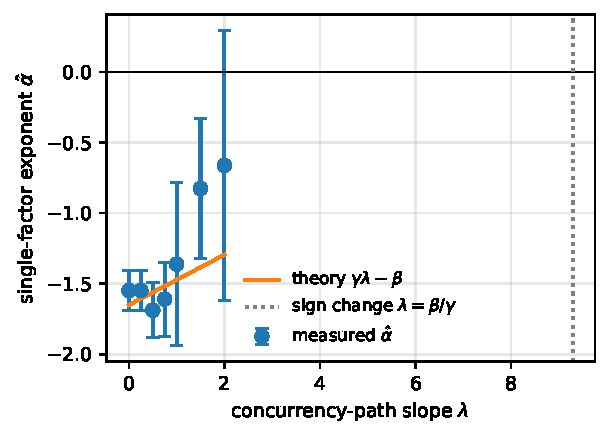
\includegraphics[width=0.75\textwidth]{figures/fig_confounding}
\caption{Experiment~X3b. Single-factor exponent $\ahat$ estimated from data
re-sampled along concurrency paths of slope~$\lambda$, against the prediction
$\gamma\lambda-\beta$ of Theorem~\ref{thm:identifiability}. The predicted sign
change is at $\lambda=\beta/\gamma=\resLambda$}
\label{fig:confounding}
\end{figure}

Figure~\ref{fig:confounding} shows the sweep: estimated exponents track the
predicted line $\gamma\lambda-\beta$. With the calibrated ratio
$\beta/\gamma=\resLambda$ the sign change lies above the concurrency paths
realized in the load-generator design, so every measured single-factor exponent
in the campaign remains negative --- yet the $\lambda=1$ point already
reproduces the classical confound of Theorem~\ref{thm:identifiability} to within
sampling error. The middle block of Table~\ref{tab:results} reports the
accompanying invariance tests: the partial $F$-test for
quota\,$\times\log\n$ interaction has $p=\resQinvP$, so exact $\q$-invariance
is rejected on the full X2 grid and the bi-factor coefficients above are
therefore reported at the reference quota $\q=0.25$ only; $\beta$ estimated
under zero and elevated round-trip time moves from $\resBetaRttZero$ to
$\resBetaRttHigh$.

\begin{table}[!t]
\centering
\caption{Calibrated parameters, invariance and detector characteristics, and
predictive coverage}
\label{tab:results}
\begin{tabular}{lll}
\headline
Quantity & Estimate & Note \\
\headline
$\Tzero$ & $\resTzero$ & normalized scale \\
$\beta$ & $\resBeta\pm\resBetaSE$ & consensus exponent \\
$\gamma$ & $\resGamma\pm\resGammaSE$ & concurrency exponent \\
$\csat$, $\theta$ & $\resCsat$, $\resTheta$ & saturation \\
$\hat\sigma$ & $\resSigmaRes$ & log-residual s.d. \\
\hline
$\ahat$ at $\lambda=0,\,1,\,2$ & $\resAlphaHatL0$, $\resAlphaHatL1$, $\resAlphaHatL2$
 & \textit{cf.}\ $\gamma\lambda-\beta$ \\
$\beta$ by quota $0.20,0.25,0.33$ & $\resBetaQlow$, $\resBetaQmid$, $\resBetaQhigh$
 & X2 \\
$q$-invariance $F$-test & $p=\resQinvP$ & Statement~\ref{st:qinvariance} \\
$\beta$ at RTT $0$, high & $\resBetaRttZero$, $\resBetaRttHigh$ & X4 \\
$\pd$, $\pf$, $\rho$ & $\resPd$, $\resPf$, $\resRho$ & at $\thr=\resDetectorThr$ \\
detector AUC & $\resAuc$ & X5 \\
\hline
held-out $\n$ & $\resHoldoutN$ & coverage set \\
coverage at $90\%$ & $\resCovNinety$ & nominal $0.90$ \\
coverage at $95\%$ & $\resCovNinetyFive$ & nominal $0.95$ \\
\headline
\end{tabular}
\end{table}

The lower block reports predictive coverage on the held-out validator counts,
which is the check that decides whether the intervals of Statement~\ref{st:pi}
may be used for sizing. An out-of-sample comparison of four predictors --- a
linear model, a single-factor power law, the Universal Scalability
Law~\cite{gunther2007} and~\eqref{eq:bifactor} --- gives held-out log-space
RMSE $\resRmseLinear$, $\resRmseSingle$, $\resRmseUsl$ and $\resRmseOurs$
respectively. The sizing ablation of Section~\ref{sec:case} further reports
relative provisioning cost under the same four predictors as
$\resCostLinear$, $\resCostSingle$, $\resCostUsl$ and $\resCostOurs$.

\section{Application to an e-governance workload, and limitations}
\label{sec:case}

We instantiate Problem~\ref{prob:sizing} on a national-scale profile:
approximately $3.0\times10^{7}$ ballots over a twelve-hour window, with a peak
window concentrating about a quarter of the daily volume and therefore a peak
demand $\Dpk\approx2.1\times10^{3}$ transactions per second. The safety
requirement is that a coordinated omission fault affecting one fifth of the
validators be detected within one epoch with probability at least $1-\epss$.

Because the bi-factor law is calibrated on \RNM{}-normalized throughput
$\TPSn=\TPS/\q$, absolute demand and the fitted law live in different units.
We therefore introduce an explicit production scale-up $\kappaScale$ such that
the absolute predictor is $\kappaScale\cdot\widehat{\TPSn}(\n,\cc)$. The default
reported here is the \emph{minimal admissible} scale: the smallest
$\kappaScale$ for which the lower prediction bound at $\n=4$ meets $\Dpk$
(hardware just capable of serving the peak at the smallest QBFT validator
set). With that $\kappaScale=\resKappa$ and operating concurrency
$\cc^{\star}=\resCstar$, Theorem~\ref{thm:window} yields the feasibility
window $[\resNminCase,\resNmaxCase]$ and the recommendation
$\nopt=\resNoptCase$; Figure~\ref{fig:window} shows the two constraints and
their intersection. Detector rates enter at the Youden-optimal participation
threshold $\thr=\resDetectorThr$ of experiment~X5.

\begin{figure}[!t]
\centering
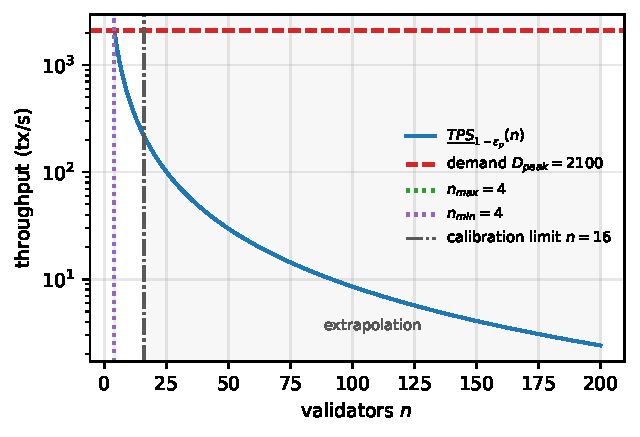
\includegraphics[width=0.78\textwidth]{figures/fig_window}
\caption{Feasibility window. The solid curve is the confidence-adjusted
absolute throughput $\kappaScale\cdot\underline{\TPSn}_{1-\epsp}(\n)$ against
the demand $\Dpk$; the shaded band marks the admissible interval
$[\nmin,\nmax]=[\resNminCase,\resNmaxCase]$ at the minimal admissible
$\kappaScale=\resKappa$}
\label{fig:window}
\end{figure}

The width of the window is the design margin, and it responds to four factors. A
relative change in $\beta$ shifts $\log\nmax$ by
$-\log\nmax\,\Delta\beta/\beta$, so the upper endpoint is most sensitive
precisely when the deployment sits far above the calibration range. Increasing
$\rho$ inflates $\nmin$ proportionally to $1+(\kf-1)\rho$
by~\eqref{eq:nmin}, so strongly coordinated faults can close the window on their
own. Using $\beta(\mathrm{RTT})$ from experiment~X4 lowers $\nmax$, which is the
price of geographic distribution. And tightening $\epsp$ lowers $\nmax$ while
tightening $\epss$ raises $\nmin$: the window closes from both sides as the
system is made more conservative. The analysis thus produces an operational
statement of the form: \emph{with confidence $1-\epsp$ the network sustains the
peak demand up to $\nmax$ validators, and detects the specified coordinated
fault with probability at least $1-\epss$ from $\nmin$ upward; the cheapest
admissible configuration is $\nopt$; the required production scale relative to
the \RNM{} unit is $\kappaScale$}.

\begin{Remark}
This case study illustrates the sizing workflow. It is not a recommendation to
conduct binding elections on a blockchain: the consensus layer addresses neither
endpoint compromise nor coercion~\cite{springall2014,specter2020,park2021}. The
same workflow applies unchanged to registry and identity workloads, where those
objections do not arise.
\end{Remark}

\subsection{Limitations}
\label{sec:limitations}

\paragraph{Fault class.}
The peer-to-peer transport is encrypted, so network-level injection cannot be
selective with respect to consensus message type. Experiment~X5 therefore
realizes omission and duplication faults only, excluding equivocation and
signature forgery, and every statement about $\pd$, $\pf$ and $\pmiss$ is
conditional on that class. Empirically, signer-metrics detection of this class
is weak (AUC~$\resAuc$ at the Youden threshold $\thr=\resDetectorThr$): the
safety constraint is consequently non-binding at the operating point of
Section~\ref{sec:case}, and the window is set by throughput.

\paragraph{Absolute throughput and measured range.}
Under the \RNM{} protocol each validator receives a small fixed CPU quota, so
absolute throughput is far below what dedicated hardware would deliver and is
not comparable with published benchmarks; every claim here concerns exponents,
coverage and the sizing decisions derived from them, and
Statement~\ref{st:qinvariance} is what licenses that separation. Absolute demand
enters the sizing problem only through the explicit scale-up $\kappaScale$ of
Problem~\ref{prob:sizing}. The largest directly measured validator set is
bounded by host memory, and extrapolation beyond it rests on the calibrated
model and on simulation; the intervals of Statement~\ref{st:pi} quantify, but
do not eliminate, the associated risk. The fitted consensus exponent
$\beta=\resBeta$ is steep, so even at the minimal admissible $\kappaScale$ the
feasibility window collapses to a single point $\n=\resNoptCase$: that is a
substantive sizing conclusion, not a numerical artefact.

\paragraph{Single host and single platform.}
All measurements come from one host and one implementation, with wide-area
behaviour emulated rather than observed. The contributions are not equally
exposed. Theorem~\ref{thm:identifiability} is a statement about least squares
and does not depend on the platform; what depends on it are the values of
$\beta$ and $\gamma$. Experiment~X9 was intended to falsify the
path-re-sampling prediction on a second QBFT-family client, but that arm of the
campaign did not produce usable records, so the numerical coefficients remain
Besu-specific. The \RNM{} protocol is more exposed, since
Assumption~\ref{as:separable} concerns the scheduler and the runtime: the X2
partial $F$-test rejects exact quota invariance on $\{0.20,0.25,0.33\}$, and we
therefore report the bi-factor fit at the reference quota $\q=0.25$ rather than
pooling across quotas.

\paragraph{Asymmetry between theory and measurement.}
The analytical part of this work is more complete than the empirical part. The
theorems hold as stated; the calibrated coefficients rest on a campaign bounded
by what a four-core runner can host, and Assumption~\ref{as:separable} in
particular is supported over a narrow quota range. The numerical values should
be read as provisional and the structural claims --- the form of the bias, the
shape of the feasible set --- as the durable part. The exchangeable correlation
of Assumption~\ref{as:rho} and the approximate log-normality underlying
Statement~\ref{st:pi} are likewise approximations, each accompanied by a test;
where a test rejects, the corresponding claim is restricted rather than
retained. Finally, Theorem~\ref{thm:window} assumes only that $\Cost$ is
nondecreasing, so deployments with non-monotone institutional cost fall outside
it, although the window itself remains valid.

\section{Conclusions}
\label{sec:conclusions}

We have addressed the problem of choosing the size of a permissioned BFT
validator set for an e-governance workload in the realistic setting where no
large testbed is available. \emph{First}, the identifiability theorem shows that
a single-factor scaling exponent converges to $\gamma\lambda-\beta$, where
$\lambda$ is a property of the measurement design rather than of the protocol; a
positive exponent is therefore consistent with a load generator scaled alongside
the network and is not by itself evidence that throughput grows with the
validator count. This offers a concrete explanation for the discrepancy between
the predictions of our earlier work~\cite{peniak2026a,peniak2026b} and indicates
which of the two designs was affected. \emph{Second}, the resource-normalized
measurement protocol fixes the per-validator compute budget independently of the
validator count, separating consensus overhead from host contention and making
the required factorial design --- and hence the theorem --- usable on a single
commodity machine; where exact $\q$-invariance is rejected, the fitted law is
reported at the reference quota. \emph{Third}, calibrated lognormal prediction
intervals,
validated by empirical coverage on held-out validator counts, replace point
accuracy figures with a falsifiable statement. \emph{Fourth}, coupling the
throughput law with a Hoeffding-type detection bound turns sizing into a
chance-constrained program whose feasible set is a closed interval
$[\nmin,\nmax]$ computable in $O(\log\n)$ evaluations, with absolute demand
entering through an explicit production scale-up $\kappaScale$; the detection
bound itself is standard, and what it contributes is a constraint monotone in the
direction opposite to throughput, so that an empty interval certifies a
structural rather than a provisioning failure.

Of the four, we regard the first as the one most likely to outlive the specific
measurements reported here, since it is a statement about estimation rather than
about any particular system. The entire campaign executes in a public
continuous-integration workflow on one four-core runner, so every result can be
reproduced without dedicated infrastructure.

\paragraph{Future work.}
Protocol-level instrumentation covering equivocation faults; validation across
several consensus implementations; extension of the feasibility window to
latency and finality constraints; and online recalibration of $\beta$ as a
deployment grows.

\subsection*{Conflict of interest}
The authors declare no conflict of interest.

\subsection*{Funding}
The research was conducted without financial support.

\subsection*{Data availability}
The workflow definition, network and load generators, fault-injection scripts,
detector, analysis code and raw measurement artefacts are available in the
project repository.

\subsection*{Use of artificial intelligence}
AI-assisted tools were used for language editing and typesetting. All scientific
results, proofs, experimental design and analysis were produced by the authors.

\subsection*{Contributions of authors}
\textbf{Peniak B.\,O.}: conceptualization, methodology, formal analysis,
software, investigation, data curation, writing --- original draft,
visualization.
\textbf{Liubinskyj B.\,B.}: supervision, validation, writing --- review and
editing.


%%%%%%%%%%%%%%%%%%%%%%%%%%%%%%%%%%%%%%%%%%%%%%%%%%%%%%%%%%%%%%%%%%%%%%%%%%%%%%%
%% bib/references.tex
%% MMC.sty redefines `thebibliography'. Do NOT use bibtex / biblatex.
%% Count: 27 entries (requirement: >= 25).
%% Every entry ends with a resolvable \url{...} (DOI preferred; open PDF/arXiv
%% when the publisher blocks automated DOI resolution).
%%%%%%%%%%%%%%%%%%%%%%%%%%%%%%%%%%%%%%%%%%%%%%%%%%%%%%%%%%%%%%%%%%%%%%%%%%%%%%%

\begin{thebibliography}{27}

%------------------------------------------------------- BFT consensus
\bibitem{castro1999}
Castro M., Liskov B. Practical Byzantine fault tolerance. Proceedings of the
Third Symposium on Operating Systems Design and Implementation (OSDI). 173--186
(1999).
\url{https://www.usenix.org/conference/osdi-99/practical-byzantine-fault-tolerance}

\bibitem{lamport1982}
Lamport L., Shostak R., Pease M. The Byzantine generals problem. ACM
Transactions on Programming Languages and Systems. \textbf{4} (3), 382--401
(1982).
\url{https://doi.org/10.1145/357172.357176}

\bibitem{dwork1988}
Dwork C., Lynch N., Stockmeyer L. Consensus in the presence of partial
synchrony. Journal of the ACM. \textbf{35} (2), 288--323 (1988).
\url{https://doi.org/10.1145/42282.42283}

\bibitem{yin2019}
Yin M., Malkhi D., Reiter M.~K., Gueta G.~G., Abraham I. HotStuff: BFT consensus
with linearity and responsiveness. Proceedings of the ACM Symposium on
Principles of Distributed Computing (PODC). 347--356 (2019).
\url{https://doi.org/10.1145/3293611.3331591}
\url{https://arxiv.org/abs/1803.05069}

\bibitem{buchman2016}
Buchman E. Tendermint: Byzantine fault tolerance in the age of blockchains.
Master's thesis, University of Guelph (2016).
\url{https://hdl.handle.net/10214/9769}

\bibitem{gilad2017}
Gilad Y., Hemo R., Micali S., Vlachos G., Zeldovich N. Algorand: scaling
Byzantine agreements for cryptocurrencies. Proceedings of the 26th Symposium on
Operating Systems Principles (SOSP). 51--68 (2017).
\url{https://doi.org/10.1145/3132747.3132757}
\url{https://arxiv.org/abs/1607.01341}

\bibitem{miller2016}
Miller A., Xia Y., Croman K., Shi E., Song D. The honey badger of BFT protocols.
Proceedings of the ACM SIGSAC Conference on Computer and Communications Security
(CCS). 31--42 (2016).
\url{https://doi.org/10.1145/2976749.2978399}
\url{https://eprint.iacr.org/2016/199}

\bibitem{vukolic2015}
Vukoli\'{c} M. The quest for scalable blockchain fabric: proof-of-work vs.\ BFT
replication. Open Problems in Network Security. IFIP AICT, vol.~468. Springer.
112--125 (2015).
\url{https://doi.org/10.1007/978-3-319-39028-4_9}

%--------------------------------------------------------- benchmarking
\bibitem{androulaki2018}
Androulaki E., et al. Hyperledger Fabric: a distributed operating system for
permissioned blockchains. Proceedings of the Thirteenth EuroSys Conference.
30:1--30:15 (2018).
\url{https://doi.org/10.1145/3190508.3190538}
\url{https://arxiv.org/abs/1801.10228}

\bibitem{thakkar2018}
Thakkar P., Nathan S., Viswanathan B. Performance benchmarking and optimizing
Hyperledger Fabric blockchain platform. 26th IEEE International Symposium on
Modeling, Analysis, and Simulation of Computer and Telecommunication Systems
(MASCOTS). 264--276 (2018).
\url{https://doi.org/10.1109/MASCOTS.2018.00034}

\bibitem{dinh2017}
Dinh T.~T.~A., Wang J., Chen G., Liu R., Ooi B.~C., Tan K.-L. BLOCKBENCH: a
framework for analyzing private blockchains. Proceedings of the ACM
International Conference on Management of Data (SIGMOD). 1085--1100 (2017).
\url{https://doi.org/10.1145/3035918.3064033}
\url{https://arxiv.org/abs/1703.04057}

\bibitem{sousa2018}
Sousa J., Bessani A., Vukoli\'{c} M. A Byzantine fault-tolerant ordering service
for the Hyperledger Fabric blockchain platform. 48th IEEE/IFIP International
Conference on Dependable Systems and Networks (DSN). 51--58 (2018).
\url{https://doi.org/10.1109/DSN.2018.00018}

%------------------------------------------------------- scaling laws
\bibitem{amdahl1967}
Amdahl G.~M. Validity of the single processor approach to achieving large scale
computing capabilities. Proceedings of the AFIPS Spring Joint Computer
Conference. 483--485 (1967).
\url{https://doi.org/10.1145/1465482.1465560}

\bibitem{gustafson1988}
Gustafson J.~L. Reevaluating Amdahl's law. Communications of the ACM.
\textbf{31} (5), 532--533 (1988).
\url{https://doi.org/10.1145/42411.42415}

\bibitem{gunther2007}
Gunther N.~J. Guerrilla capacity planning: a tactical approach to planning for
highly scalable applications and services. Springer (2007).
\url{https://doi.org/10.1007/978-3-540-31010-5}

%----------------------------------------------- concentration, statistics
\bibitem{hoeffding1963}
Hoeffding W. Probability inequalities for sums of bounded random variables.
Journal of the American Statistical Association. \textbf{58} (301), 13--30
(1963).
\url{https://doi.org/10.1080/01621459.1963.10500830}

\bibitem{boucheron2013}
Boucheron S., Lugosi G., Massart P. Concentration inequalities: a nonasymptotic
theory of independence. Oxford University Press (2013).
\url{https://doi.org/10.1093/acprof:oso/9780199535255.001.0001}

\bibitem{efron1993}
Efron B., Tibshirani R.~J. An introduction to the bootstrap. Chapman and Hall
(1993).
\url{https://doi.org/10.1201/9780429246593}

\bibitem{seber2003}
Seber G.~A.~F., Wild C.~J. Nonlinear regression. Wiley (2003).
\url{https://doi.org/10.1002/0471725315}

%------------------------------------ optimization under uncertainty
\bibitem{charnes1959}
Charnes A., Cooper W.~W. Chance-constrained programming. Management Science.
\textbf{6} (1), 73--79 (1959).
\url{https://doi.org/10.1287/mnsc.6.1.73}

\bibitem{nemirovski2007}
Nemirovski A., Shapiro A. Convex approximations of chance constrained programs.
SIAM Journal on Optimization. \textbf{17} (4), 969--996 (2006/2007).
\url{https://doi.org/10.1137/050622328}
\url{https://optimization-online.org/wp-content/uploads/2004/12/1033.pdf}

%--------------------------------------------- e-governance, e-voting
\bibitem{springall2014}
Springall D., Finkenauer T., Durumeric Z., Kitcat J., Hursti H., MacAlpine M.,
Halderman J.~A. Security analysis of the Estonian internet voting system.
Proceedings of the ACM SIGSAC Conference on Computer and Communications Security
(CCS). 703--715 (2014).
\url{https://doi.org/10.1145/2660267.2660315}
\url{https://jhalderm.com/pub/papers/ivoting-ccs14.pdf}

\bibitem{specter2020}
Specter M.~A., Koppel J., Weitzner D. The ballot is busted before the
blockchain: a security analysis of Voatz. Proceedings of the 29th USENIX
Security Symposium. 1535--1553 (2020).
\url{https://www.usenix.org/system/files/sec20-specter.pdf}

\bibitem{park2021}
Park S., Specter M., Narula N., Rivest R.~L. Going from bad to worse: from
internet voting to blockchain voting. Journal of Cybersecurity. \textbf{7} (1),
tyaa025 (2021).
\url{https://doi.org/10.1093/cybsec/tyaa025}

%------------------------------------------------------------- tooling
\bibitem{besu}
Hyperledger Besu documentation. Hyperledger Foundation.
\url{https://github.com/hyperledger/besu}
\url{https://www.hyperledger.org/use/besu}

%--------------------------------------------------------- own prior work
\bibitem{peniak2026a}
Peniak B.~O., Liubinskyj B.~B., Solomka I.~R. Minimal-sample performance
prediction for Byzantine consensus: the $\alpha$-calibration method.
Mathematical Modeling and Computing. (accepted; to appear) (2026).
\url{https://science.lpnu.ua/mmc}

\bibitem{peniak2026b}
Peniak B.~O., Liubinskyj B.~B. Adaptive hybrid consensus mechanism for
blockchain-based e-governance: a machine learning approach. Scientific Bulletin
of Uzhhorod University. Series of Mathematics and Informatics. \textbf{49} (2),
255--261 (2026).
\url{https://doi.org/10.24144/2616-7700.2026.49(2).255-261}

\end{thebibliography}


\maketitleUkr

\end{document}
